
                                                                                                                                                                                                                                                                                                                                                                                                                                                                                                                                                                                                                                                                                                                                                                                                                                                                                                                                                                                                                                                                                                                                                                                                                                                                                                                                                                                                                                                                                                                                                                                                                                                                                                                                                                                                                                                                                                                                                                                                                                                                                                                                                                                                                                                                                                                                                                                                                                                                                                                                                                                                                                                                                                                                                                                                                                                                                                                                                                                                                                                                                                                                                                                                                                                                                                                                                                                                                                                                                                                                                                                                                                                                                                                                                                                                                                                                                                                                                                                                                                                                                                                                                                                                                                                                                                                                                                                                                                                                                                                                                                                                                                                                                                                                                                                                                                                                                                                                                                                                                                                                                                                                                                                                                                                                                                                                                                                                                                                                                                                                                                                                                                                                                                                                                                                                                                                                                                                                                                                                                                                                                                                                                                                                                                                                                                                                                                                                                                                                                                                                                                                                                                                                                                                                                                                                                                                                                                                                                                                             %2multibyte Version: 5.50.0.2890 CodePage: 65001
%\input{tcilatex}
%\input{tcilatex}
%\input{tcilatex}
%\input{tcilatex}


\documentclass[notes=show]{beamer}
%%%%%%%%%%%%%%%%%%%%%%%%%%%%%%%%%%%%%%%%%%%%%%%%%%%%%%%%%%%%%%%%%%%%%%%%%%%%%%%%%%%%%%%%%%%%%%%%%%%%%%%%%%%%%%%%%%%%%%%%%%%%%%%%%%%%%%%%%%%%%%%%%%%%%%%%%%%%%%%%%%%%%%%%%%%%%%%%%%%%%%%%%%%%%%%%%%%%%%%%%%%%%%%%%%%%%%%%%%%%%%%%%%%%%%%%%%%%%%%%%%%%%%%%%%%%
\usepackage{mathpazo}
\usepackage{hyperref}


\usepackage{graphicx}
%\usepackage[spanish]{babel}
\usepackage[latin1]{inputenc}
\usepackage{listings}
\usepackage{amsmath}
\usepackage{amsfonts}
\usepackage{amsxtra}
\usepackage{amstext}
\usepackage{amssymb}
\usepackage{latexsym}
\usepackage{subfigure}
\usepackage{eurosym}
\linespread{1.2}
\usepackage{multimedia}
\usepackage{dsfont} % for \mathds{N}
\usepackage{graphicx}
\usepackage{color,colortbl}
\usepackage{multirow}
\definecolor{clearBlue}{cmyk}{0.15,0.1,0,0.1}
\usepackage{bbm}

%TCIDATA{OutputFilter=LATEX.DLL}
%TCIDATA{Version=5.50.0.2890}
%TCIDATA{Codepage=65001}
%TCIDATA{<META NAME="SaveForMode" CONTENT="1">}
%TCIDATA{BibliographyScheme=Manual}
%TCIDATA{LastRevised=Sunday, April 01, 2012 14:26:41}
%TCIDATA{<META NAME="GraphicsSave" CONTENT="32">}

\newenvironment{stepenumerate}{\begin{enumerate}[<+->]}{\end{enumerate}}
\newenvironment{stepitemize}{\begin{itemize}[<+->]}{\end{itemize} }
\newenvironment{stepenumeratewithalert}{\begin{enumerate}[<+-| alert@+>]}{\end{enumerate}}
\newenvironment{stepitemizewithalert}{\begin{itemize}[<+-| alert@+>]}{\end{itemize} }
\usetheme{Singapore}

%\input{tcilatex}

\begin{document}

\title[Moment Inequalities]{Applications of Moment Inequalities:\\ Ho (2009) }
\author[MJ Dickstein]{Michael J. Dickstein \\
%EndAName
Stanford University}
\institute{Economics 258}
%\date[3/11/13]{March 11, 2013}
\maketitle

%--------------------------------------------------------------------------------

\section{Inference}

%%%%%%%%%%%%%%%%%%%%%%%%

\begin{frame}
\frametitle{Identified Set}

\begin{itemize}
\item Moment inequalities will generically lead to set identification. Given
a set $S$ of moment inequalities, the identified set is:  
\begin{equation*}
\Theta^{S}=\operatornamewithlimits{argmin}_{\theta}\sum_{s=1}^{S}\Big(\min%
\big\{0,\mathbbm{E}[m_{s}(Y,X,Z;\theta)]\big\}\Big)^{2}
\end{equation*}
\begin{figure}[h!]
\begin{center}
\subfigure{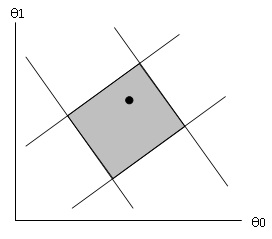
\includegraphics[scale=0.65]{Figure_1.jpg}}  \subfigure{%
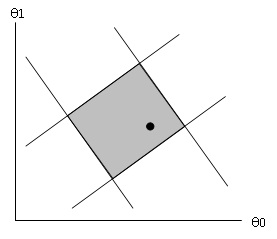
\includegraphics[scale=0.65]{Figure_2.jpg}} 
\end{center}
\end{figure}
\end{itemize}
\end{frame}

%%%%%%%%%%%%%%%%%%%%%%%%

\begin{frame}
\frametitle{Steps for Estimation}

\begin{itemize}
\item Step 1: Estimate the identified set given sample moments. 

\item Step 2: Perform inference on one or more of the following parameters: 

\begin{itemize}
\item Interval contained in the identified set: Pakes, Porter, Ho and Ishii
(2011). 

\item Identified set: Chernozhukov, Hong and Tamer (Econometrica, 2007). 

\item True parameter vector: Andrews and Soares (Econometrica, 2010). 
\end{itemize}
\end{itemize}
\end{frame}


%%%%%%%%%%%%%%%%%%%%%%%%%

\begin{frame}
\frametitle{Set/Point Inference: General Intuition}

\begin{itemize}
\item Based on the inversion of an Anderson-Rubin T statistic. 

\item General steps in the algorithm: 

\begin{enumerate}
\item Define $\theta $ grids, $\widehat{\Theta }_{n}^{Grid}$ and $\widehat{%
\Theta }_{n}^{\epsilon }$, where $\widehat{\Theta }_{n}^{\epsilon }\subset 
\widehat{\Theta }_{n}^{Grid}$. 

\item Calculate $T_{r}(\theta )$, at a set of points in either $\widehat{%
\Theta }_{n}^{Grid}$ or $\widehat{\Theta }_{n}^{\epsilon }$ depending on
whether the focus of inference is the identified set or the true value of
the parameter. 

\item Determine a critical value as a quantile of $T_{r}(\theta)$ for $%
r=1,...,R$ 

\item Calculate $T^{obs}(\theta )$ at each $\theta \in \widehat{\Theta }%
_{n}^{Grid}$ with the observed data for all moments. 

\item Define the confidence set as those $\theta$ points where $%
T^{obs}(\theta)$ falls below the critical value. 
\end{enumerate}
\end{itemize}
\end{frame}

%%%%%%%%%%%%%%%%%%%%%%%%%

\begin{frame}
\frametitle{Forming the Grids: $\widehat{\Theta}_{I}^{Grid}$ and
$\widehat{\Theta}_{I}^{\epsilon}$}

$\widehat{\Theta }_{n}^{\epsilon }\subset \widehat{\Theta }_{n}^{Grid}$

\begin{figure}[h!]
\begin{center}
\subfigure{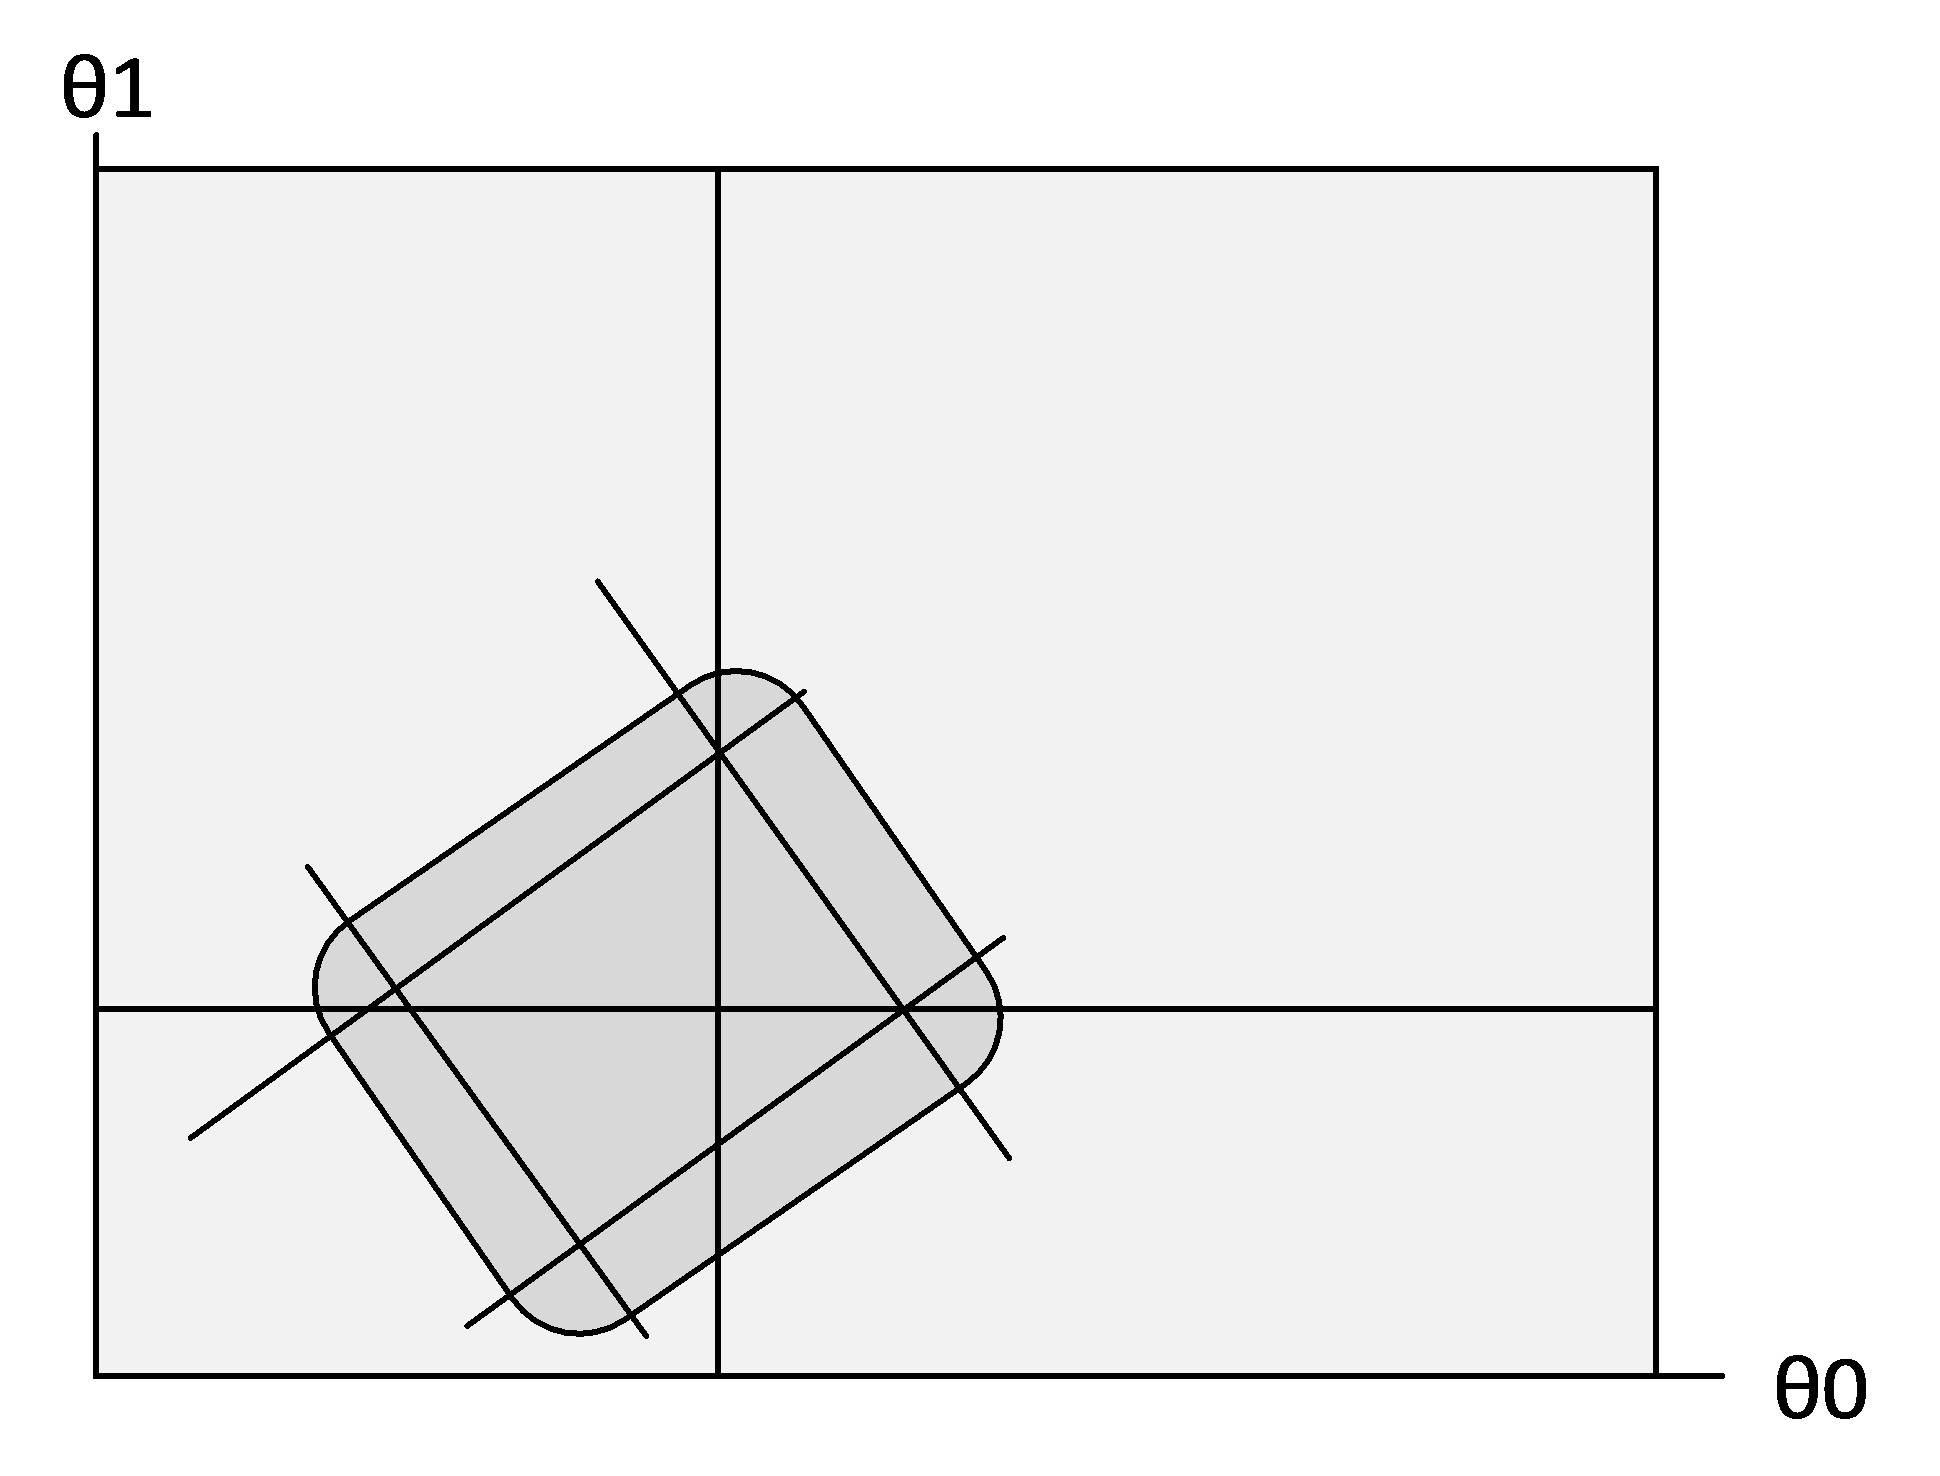
\includegraphics[scale=0.18]{Figure_9.jpg}}
\end{center}
\end{figure}
\end{frame}

%--------------------------------------------------------------------------------
\section{Ho 2009}
%--------------------------------------------------------------------------------

\begin{frame}
\frametitle{Ho 2009}

\begin{itemize}
	\item Theory testing
	\item Measurement
	\item Methodology
\end{itemize}
\end{frame}

%--------------------------------------------------------------------------------

\begin{frame}
\frametitle{Ho 2009}

\begin{itemize}
	\item Theory testing
         \begin{itemize}
	\item Can a bargaining model explain the hospital-insurance plan contracting process, rationalizing the observed network of hospital-plan relationships? 	\end{itemize}
	\item Measurement
	\begin{itemize}
	\item What characteristics of hospitals and plans explain the level of surplus hospitals can extract from the relationship?
	\item What is the effect of capacity constraints on producer welfare?  Might the level of capacity be a relevant choice variable for a profit-maximizing firm?
	\end{itemize}
\end{itemize}
\end{frame}

%--------------------------------------------------------------------------------

\begin{frame}
\frametitle{Ho 2009}

\begin{itemize}
	\item Methodology
	\begin{itemize}
	\item What assumptions are needed on behavior to develop a moment inequality estimator for static contracting problems?
	\item What can information on ex-post network formation reveal about private negotiated prices?
	\end{itemize}
\end{itemize}
\end{frame}

%--------------------------------------------------------------------------------

\begin{frame}
\frametitle{Ho 2009}

Main Idea
\begin{itemize}
	\item Model demand for hospitals and health plans, accounting for the hospital network of each plan in the consumer`s plan choice
	\item Model the supply side negotiation between hospitals and plans in forming equilibrium networks, which determines the division of profits
        \item To increase their share of the surplus from contracting, hospitals have incentives to:
         \begin{itemize}
	\item Invest in quality to attract more patients, lower costs
	\item Merge with other providers, to improve bargaining position
	\item Under-invest in capacity
	\end{itemize}
\end{itemize}
\end{frame}

%--------------------------------------------------------------------------------

\begin{frame}
\frametitle{Ho 2009}

Main Idea
\begin{itemize}
\item Findings
\begin{itemize}
\item ``Star`` hospitals capture \$6700 more per patient than other providers, on costs of \$11,000
\item Hospitals with capacity constraints have markups of \$6900 per patient more than those without constraints
\item System hospitals have \$180,000/month greater profits than other providers
\end{itemize}
\end{itemize}
\end{frame}

%--------------------------------------------------------------------------------
\begin{frame}
\frametitle{Ho 2009}

Model: Stages
\begin{itemize}
\item 0. Plans choose quality and products; Hospitals choose capacity, location, product mix, system mergers.
\item 1. Hospitals make simultaneous take-it-or-leave-it price offers to all plans in the market
\item 2. Plans choose whether to accept these offers, forming their hospital network
\item 3. Plans set premiums to maximize profits after a change in networks
\item 4. Consumers and employers jointly choose plans
\item 5. Sick consumers visit hospitals; plans pay hospitals per service provided.
\end{itemize}
\end{frame}

%--------------------------------------------------------------------------------
\begin{frame}
\frametitle{Ho 2009}

Model: Negotiation
\begin{itemize}
\item All hospitals make TIOLI offers of \{contract,null offer\}
\item All plans simultaneously respond
\item Offers are private info; plans have passive beliefs (if plan gets an alternative offer from h, doesn't change plan's beliefs about offers h makes to its competitors)

\[
\pi _{j,m}^{P} =S_{j,m}(H_{j},H_{-j})-c_{j,m}^{Hosp}(H_{j},H_{-j},X,\theta
)-c_{j,m}^{nonhosp}(H_{j},H_{-j},X,\theta )
\]
\begin{eqnarray*}
\pi _{j,m}^{P,o}(.) &=&\pi _{j,m}^{P}+\mu _{j,H_{j}} \\
E[\pi _{j,m}^{P}(H_{j},H_{-j},X,\theta )|Ij,m] &=&\pi
_{j,m}^{P}(H_{j},H_{-j},X,\theta )-\varphi _{j,H_{j}}
\end{eqnarray*}

\end{itemize}

\end{frame}

%--------------------------------------------------------------------------------
\begin{frame}
\frametitle{Ho 2009}

Model: Negotiation
\begin{itemize}
\item Key assumption: plan j`s expected profits from $H_{j}$ $>$ expected profits from alternative network formed by reversing contract with h
\[
E[\pi _{j,m}^{P,o}(H_{j},H_{-j},X,\theta )-\pi
_{j,m}^{P,o}(H_{j}^{h},H_{-j},X,\theta )|Z_{j,m}]\geq 0
\]
\item form unconditional moments using positive-valued function of $Z_{j,m}$
\begin{itemize}
\item must be known to firms when they make their choice
\item use char in fixed cost and markup terms other than cost/admission
\item use indicators for some plan and market characteristics
\end{itemize}

\end{itemize}

\end{frame}

%--------------------------------------------------------------------------------
\begin{frame}
\frametitle{Ho 2009}

Model: Negotiation
\begin{itemize}
\item Choose counterfactuals of reversing a single contract.
\item Plans may respond by changing its response to other hospital`s offers (passive beliefs rules out the following: plan responds to changes in h`s offer by assuming other plans have different offers and therefore change their own networks)
\end{itemize}

\end{frame}
%--------------------------------------------------------------------------------

\end{document}
